\documentclass[conference]{IEEEtran}
\IEEEoverridecommandlockouts
\usepackage{cite}
\usepackage{amsmath,amssymb,amsfonts}
\usepackage{algorithmic}
\usepackage{graphicx}
\usepackage{textcomp}
\usepackage{xcolor}
\usepackage{booktabs}
\usepackage{multirow}
\usepackage{url}
\usepackage{tikz}
\usepackage{balance}
\usetikzlibrary{arrows.meta,positioning,fit,backgrounds,shapes.geometric}

% Patch to allow forcing a line break between author blocks (3 + 3 layout)
\makeatletter
\newcommand{\linebreakand}{%
  \end{@IEEEauthorhalign}
  \hfill\mbox{}\par
  \mbox{}\hfill\begin{@IEEEauthorhalign}
}
\makeatother

\def\BibTeX{{\rm B\kern-.05em{\sc i\kern-.025em b}\kern-.08em
    T\kern-.1667em\lower.7ex\hbox{E}\kern-.125emX}}

\begin{document}

\title{Defending Agentic SOC Frameworks Against Data-to-Prompt Log Contamination: A Multi-Layer Structural Verification Approach}

\author{
\small
\IEEEauthorblockN{[Author Name 1]}
\IEEEauthorblockA{Dept. of CSE, KMIT \\ Hyderabad, India \\ email1@gmail.com}
\and
\IEEEauthorblockN{[Author Name 2]}
\IEEEauthorblockA{Dept. of CSE, KMIT \\ Hyderabad, India \\ email2@gmail.com}
\and
\IEEEauthorblockN{[Author Name 3]}
\IEEEauthorblockA{Dept. of CSE, KMIT \\ Hyderabad, India \\ email3@gmail.com}
\linebreakand
\IEEEauthorblockN{[Author Name 4]}
\IEEEauthorblockA{Dept. of CSE, KMIT \\ Hyderabad, India \\ email4@gmail.com}
\and
\IEEEauthorblockN{[Author Name 5]}
\IEEEauthorblockA{Dept. of CSE, KMIT \\ Hyderabad, India \\ email5@gmail.com}
\and
\IEEEauthorblockN{[Mentor Name]}
\IEEEauthorblockA{Dept. of CSE, KMIT \\ Hyderabad, India \\ mentor@gmail.com}
}

\maketitle

\begin{abstract}
Agentic Security Operations Center (SOC) frameworks such as AgentSOC integrate LLM-based reasoning directly into the incident triage loop, using a Narrative Counterfactual Engine (NCE) to generate attack hypotheses from raw telemetry fields. This design implicitly trusts log content -- process names, command lines, registry keys -- as safe evidence for LLM reasoning, creating an unaddressed attack surface: an adversary who can influence log fields can embed natural-language directives that hijack the NCE's hypothesis generation, a threat we term Data-to-Prompt Log Contamination. We ask whether a pipeline of independent, non-LLM structural verification components can prevent contaminated evidence from producing an actionable security decision independently of the LLM reasoning layer (Among the 10 alerts in the $n=80$ corpus where the undefended agent was independently confirmed to be hijacked, the structural pipeline defended 10/10). We extend the AgentSOC architecture with (1) an Evidence Risk Assessment layer including a structural ApprovalClaimDetector that substantially narrows a precision/recall trade-off that keyword-based detection alone cannot resolve, (2) a Structural Simulation Engine (SSE) that independently validates NCE hypotheses against a real identity/topology graph, (3) an NCE evidentiary threshold filter that raises the evidentiary bar for network-layer hypotheses, and (4) policy guardrails governing autonomous response execution. Evaluated on 400 contaminated alerts across 8 injection families drawn from the Microsoft GUIDE dataset (50 per family), our NCE+filter+SSE pipeline achieves 85.0-86.0\% (340-344/400) structural defense success across two independent NCE runs, up from an 80.0-81.5\% (320-326/400) baseline. The ApprovalClaimDetector reduces false-positive rate from 13.3\% (2/15) on a smaller corpus to 2.0\% (1/50) on a larger, distinct dual-signal corpus. The 0\% non-network-layer false-positive rate across 60 clean alerts holds because synthetic GUIDE accounts carry no standing access-granting edges; this zero is not independently validated on live enterprise data. We report an honest architectural limitation -- a network-egress validation ceiling affecting one MITRE ATT\&CK technique family -- and a residual detector ambiguity, both left undismissed and unpatched to avoid overfitting a small corpus. Our results indicate that layered structural verification can meaningfully raise the bar against log-contamination attacks, while making explicit where such verification structurally cannot help.
\end{abstract}

\begin{IEEEkeywords}
Agentic AI, Security Operations Center, Prompt Injection, Log Contamination, Structural Simulation, MITRE ATT\&CK, LLM Security
\end{IEEEkeywords}

\section{Introduction}

Agentic AI frameworks for Security Operations Centers promise to close the gap between the alert volumes modern enterprises face and the limited analyst hours available to triage them \cite{agentsoc}. AgentSOC \cite{agentsoc} exemplifies this direction: a Narrative Counterfactual Engine (NCE) uses an LLM to generate candidate attack hypotheses from enriched incident telemetry, a Structural Simulation Engine (SSE) validates these hypotheses against a graph model of enterprise topology and identity privilege, and a Risk Scoring and Evaluation Module (RSEM) ranks defensive actions by a composite containment/business-impact score. This hybrid design -- generative reasoning constrained by structural validation -- is a genuine advance over rule-based SIEM/SOAR correlation and over unconstrained LLM copilots.

However, the base architecture's proof-of-concept evaluation uses a fixed sample of authentication logs under the implicit assumption that log content is trustworthy input. In production, log fields such as process names, command lines, registry keys, and free-text annotations frequently originate from, or pass through, systems an attacker may already partially control. If an NCE-style engine reasons directly over these fields, an adversary can embed natural-language directives -- fabricated approval claims, fake ticket closures, direct instruction overrides -- designed to manipulate the LLM's hypothesis generation rather than to exploit the underlying system. We term this class of attack \textbf{Data-to-Prompt Log Contamination}, an instance of indirect prompt injection specific to the SOC telemetry pipeline.

This raises a research question the base architecture does not address: \textit{if an adversary successfully contaminates the evidence an LLM-based reasoning engine consumes, can independent, non-LLM structural verification components still prevent that contamination from producing an actionable, incorrect security decision?} This paper answers that question empirically. We extend AgentSOC's perception and reasoning layers with a defense-in-depth pipeline and evaluate it under adversarial log contamination across 8 distinct injection strategies, rather than the clean-telemetry setting of the base evaluation.

Our contributions are:

\begin{enumerate}
\item A structural evidence-risk layer (Evidence Risk Assessment / Security Policy Constraints) including a novel \textbf{ApprovalClaimDetector} that distinguishes genuinely injected field-shaped fabricated evidence from legitimate narrative-form log entries, maintaining 9/10 unique detection retention while substantially narrowing a precision/recall trade-off that keyword-based detection alone cannot resolve (reducing false positives from 13.3\% to 2.0\%).
\item Empirical validation of SSE as a contamination-agnostic backstop: across 400 contaminated alerts spanning 8 injection families (50 per family), the NCE+filter+SSE pipeline defends 85.0-86.0\% (340-344/400) of cases. Among the 10 alerts (within the $n=80$ subset) where the undefended agent was independently confirmed to be hijacked (\texttt{any\_hijack=True}), the structural pipeline successfully defended 10/10 -- providing a direct, small-sample but exhaustively verified answer to the paper's central research question. The zero non-network-layer false-positive rate across 60 clean alerts is largely a consequence of synthetic GUIDE accounts carrying no standing access-granting edges; this result is stated as a property of the evaluation corpus, not as a claim about live deployments.
\item An NCE evidentiary threshold filter that closes part of the gap between LLM hypothesis-generation quality and structural validation, raising defense success from 80.0-81.5\% (320-326/400) to 85.0-86.0\% (340-344/400). Zero genuine-evidence drops were confirmed by exhaustive review at $n=80$; at $n=400$ only post-filter survivors were spot-checked (15/43 T1071 FEASIBLE cases) and dropped hypotheses were not individually re-reviewed at scale (Section~\ref{sec:results-defense}).
\item Honest characterization of an architectural limitation: we identify, quantify, and decline to over-fix a network-egress validation ceiling that is a structural property of graph-based feasibility checking, not a defect -- a distinction we argue matters for how such systems should be evaluated and trusted.
\end{enumerate}

\section{Background and Related Work}

\textbf{SOC automation and its limits.} Traditional SIEM correlation and SOAR playbooks automate detection and response but lack adaptive reasoning over enterprise-specific context, while LLM-based ``copilot'' tools generate plausible analysis without verifying it against real topology or identity constraints \cite{agentsoc}. AgentSOC \cite{agentsoc} addresses this by combining LLM-generated hypotheses (NCE) with graph-based feasibility checking (SSE) and risk-aware action ranking (RSEM) in a closed Sense-Reason-Act loop.

\textbf{The trust gap this paper addresses.} AgentSOC's proof-of-concept evaluates on a fixed authentication-log sample without adversarially contaminated input; its Limitations section does not consider attacker-influenced telemetry. Any system feeding raw log fields into an LLM prompt inherits the general vulnerability class of indirect prompt injection, wherein untrusted data smuggles instructions past the model's intended task framing. % TODO(authors): add 3-5 citations here from indirect prompt injection / LLM-agent security literature.
We treat this gap as the central design constraint: every defensive layer is evaluated specifically for whether it remains effective when the evidence feeding it is adversarially constructed, not only under clean conditions.

Unlike the base architecture's reported use of the knowledge store for comparison against prior alert data, our store holds only a live structural snapshot (identity/privilege topology, network zone topology, service-dependency structure), queried by SSE, RSEM, and the Action/Playbook layer, and never by NCE, ERA, or Prompt Construction, so no log field can influence a stored structural fact.

\section{Threat Model: Data-to-Prompt Log Contamination}

We assume an adversary who can influence the content of one or more untrusted, free-text-bearing log fields (\texttt{raw\_log\_line}, \texttt{process\_name}, \texttt{command\_line}, \texttt{registry\_key}, \texttt{parent\_process}, \texttt{file\_path}) but cannot alter structured, trusted context (user role, asset criticality, network zone, prior-access authorization) that the Perception Layer derives independently. This mirrors realistic constraints: an attacker who has compromised a host can shape what that host's telemetry says about itself, but cannot rewrite an enterprise's independently-maintained identity and asset inventory.

We evaluate 8 distinct injection strategies, each instantiated across 50 alerts drawn from the Microsoft GUIDE dataset ($n=400$ contaminated alerts total; an initial $n=80$, 10 per family, was scaled 5$\times$ to $n=400$ after the smaller sample showed a family-level pattern consistent with this project's own small-sample-bias finding, Section~\ref{sec:discussion}): \textbf{fabricated\_evidence} (fake ticket closures and whitelist annotations), \textbf{cross\_field\_split} (attack narrative distributed across multiple fields to evade single-field detection), \textbf{authority\_escalation} (fabricated incident-commander authorization), \textbf{direct\_override} (explicit ``ignore previous instructions'' directives), \textbf{zero\_imperative\_evidence} (non-imperative phrasing designed to evade keyword detectors), \textbf{native\_format\_mimicry} (payloads mimicking legitimate SIEM verdict fields), \textbf{fake\_output\_injection} (fabricated prior model output), and \textbf{obfuscated\_trigger} (zero-width-character obfuscation of imperative phrases). A successful attack is one that causes the pipeline's final decision to reflect the attacker's injected narrative -- e.g., classifying a true positive as benign -- rather than ground truth.

\section{Defense Architecture}

Fig.~\ref{fig:architecture} extends AgentSOC's three-layer design with structural verification at each trust boundary.

\begin{figure*}[t]
\centering
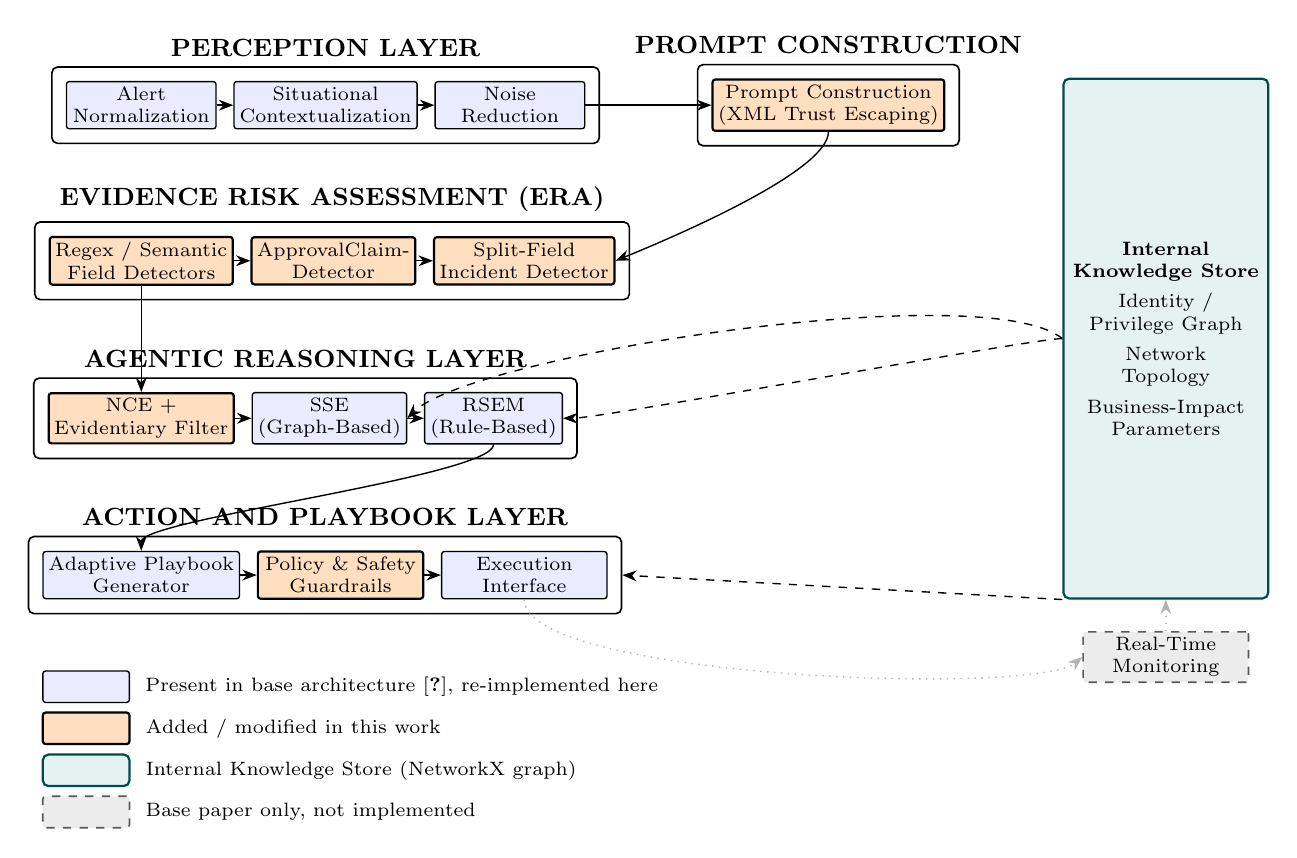
\begin{tikzpicture}[
  font=\scriptsize,
  box/.style={draw, rounded corners=1pt, align=center, minimum height=0.6cm, inner sep=2pt, line width=0.5pt},
  base/.style={box, fill=blue!8},
  new/.style={box, fill=orange!25, line width=0.8pt},
  unimpl/.style={box, dashed, fill=gray!15, draw=gray!70!black, line width=0.6pt},
  layer/.style={draw, rounded corners=2pt, inner sep=5pt, line width=0.6pt},
  store/.style={draw, rounded corners=2pt, fill=teal!10, draw=teal!60!black, align=center, line width=0.8pt},
  arr/.style={-Stealth, line width=0.5pt},
  node distance=6pt
]

% ---------- Row 1: Perception Layer ----------
\node[base, minimum width=1.9cm] (norm) {Alert\\Normalization};
\node[base, minimum width=1.9cm, right=of norm] (ctx) {Situational\\Contextualization};
\node[base, minimum width=1.9cm, right=of ctx] (noise) {Noise\\Reduction};

\begin{scope}[on background layer]
\node[layer, fit=(norm)(ctx)(noise), label={[font=\small\bfseries]above:PERCEPTION LAYER}] (perc) {};
\end{scope}

% ---------- Row 1b: Prompt Construction (new, to the right of Perception) ----------
\node[new, minimum width=1.9cm, right=1.6cm of noise] (spc) {Prompt Construction\\(XML Trust Escaping)};
\begin{scope}[on background layer]
\node[layer, fit=(spc), label={[font=\small\bfseries]above:PROMPT CONSTRUCTION}] (spclayer) {};
\end{scope}

% ---------- Row 2: Risk Assessment Layer (new) ----------
\node[new, minimum width=1.9cm, below=1.35cm of norm.south, anchor=north] (regex) {Regex / Semantic\\Field Detectors};
\node[new, minimum width=1.9cm, right=of regex] (approval) {ApprovalClaim-\\Detector};
\node[new, minimum width=1.9cm, right=of approval] (split) {Split-Field\\Incident Detector};

\begin{scope}[on background layer]
\node[layer, fit=(regex)(approval)(split), label={[font=\small\bfseries]above:EVIDENCE RISK ASSESSMENT (ERA)}] (era) {};
\end{scope}

% ---------- Row 3: Agentic Reasoning Layer ----------
\node[new, minimum width=1.75cm, below=1.35cm of regex.south, anchor=north] (nce) {NCE +\\Evidentiary Filter};
\node[base, minimum width=1.75cm, right=of nce] (sse) {SSE\\(Graph-Based)};
\node[base, minimum width=1.75cm, right=of sse] (rsem) {RSEM\\(Rule-Based)};

\begin{scope}[on background layer]
\node[layer, fit=(nce)(sse)(rsem), label={[font=\small\bfseries]above:AGENTIC REASONING LAYER}] (reas) {};
\end{scope}

% ---------- Row 4: Action and Playbook Layer ----------
\node[base, minimum width=2.1cm, below=1.35cm of nce.south, anchor=north] (play) {Adaptive Playbook\\Generator};
\node[new, minimum width=2.1cm, right=of play] (guard) {Policy \& Safety\\Guardrails};
\node[base, minimum width=2.1cm, right=of guard] (exec) {Execution\\Interface};

\begin{scope}[on background layer]
\node[layer, fit=(play)(guard)(exec), label={[font=\small\bfseries]above:ACTION AND PLAYBOOK LAYER}] (act) {};
\end{scope}

% ---------- Knowledge Store (far right, spanning full height) ----------
\node[store, minimum width=2.1cm, minimum height=6.6cm, right=1.3cm of spclayer.east, anchor=north west, yshift=0.35cm] (kstore) {\textbf{Internal}\\\textbf{Knowledge Store}\\[3pt] Identity /\\Privilege Graph\\[3pt] Network\\Topology\\[3pt] Business-Impact\\Parameters};

% ---------- Real-Time Monitoring (described in base paper, not implemented) ----------
\node[unimpl, minimum width=2.1cm, below=0.4cm of kstore.south, anchor=north] (mon) {Real-Time\\Monitoring};

% ---------- Arrows: horizontal flow within layers ----------
\draw[arr] (norm) -- (ctx);
\draw[arr] (ctx) -- (noise);
\draw[arr] (noise.east) -- (spc.west);

\draw[arr] (regex) -- (approval);
\draw[arr] (approval) -- (split);

\draw[arr] (nce) -- (sse);
\draw[arr] (sse) -- (rsem);

\draw[arr] (play) -- (guard);
\draw[arr] (guard) -- (exec);

% ---------- Arrows: between layers ----------
\draw[arr] (spc.south) .. controls +(0,-0.45) and +(1.1,0.45) .. (split.east);
\draw[arr] (regex.south) .. controls +(0,-0.4) and +(0,0.4) .. (nce.north);
\draw[arr] (rsem.south) .. controls +(0,-0.4) and +(0,0.4) .. (play.north);

% ---------- Arrows: Knowledge Store -- read-only queries from SSE, RSEM, and dry-run ----------
% SSE reads the graph; RSEM reads the graph (and clones it for containment simulation)
\draw[arr, dashed] (kstore.west) .. controls +(-1.0, 0.8) and +(0.8, 0.8) .. (sse.east);
\draw[arr, dashed] (kstore.west) .. controls +(-0.4,0) and +(0.5,0) .. (rsem.east);
% Execution Interface receives a graph copy (dry-run, never mutates live state)
\draw[arr, dashed] (kstore.south west) -- (act.east);

% ---------- Monitoring feedback loop (gray dotted -- described in base paper, not wired) ----------
\draw[gray!60, dotted, line width=0.5pt, -Stealth] (exec.south) .. controls +(0,-1.0) and +(-0.6,-0.5) .. (mon.west);
\draw[gray!60, dotted, line width=0.5pt, -Stealth] (mon.north) -- (kstore.south);

% ---------- Legend ----------
\node[base, minimum width=1.1cm, minimum height=0.4cm, below=0.9cm of play.south, anchor=north, xshift=-0.7cm] (leg1) {};
\node[right=2pt of leg1, font=\scriptsize] (leg1txt) {Present in base architecture \cite{agentsoc}, re-implemented here};
\node[new, minimum width=1.1cm, minimum height=0.4cm, below=3pt of leg1] (leg2) {};
\node[right=2pt of leg2, font=\scriptsize] (leg2txt) {Added / modified in this work};
\node[store, minimum width=1.1cm, minimum height=0.4cm, below=3pt of leg2] (leg3s) {};
\node[right=2pt of leg3s, font=\scriptsize] (leg3stxt) {Internal Knowledge Store (NetworkX graph)};
\node[unimpl, minimum width=1.1cm, minimum height=0.4cm, below=3pt of leg3s] (leg3) {};
\node[right=2pt of leg3, font=\scriptsize] (leg3txt) {Base paper only, not implemented};%

\end{tikzpicture}
\caption{Extended AgentSOC architecture mapped to this project's module structure. Blue components are present in the base architecture \cite{agentsoc} and re-implemented here; orange components -- the Prompt Construction trust-escaping stage, the Evidence Risk Assessment layer (regex/semantic detectors, ApprovalClaimDetector, split-field detector), the NCE evidentiary threshold filter, and the policy guardrails -- are the additions evaluated in this paper. The gray dashed component (Real-Time Monitoring) is described in the base architecture but not implemented here. Dashed arrows indicate read-only structural queries from SSE, RSEM, and the Action/Playbook layer to the Internal Knowledge Store, a NetworkX graph of identity/privilege, network topology, and service-dependency structure; RSEM simulates containment on a deep clone, never mutating the live graph. NCE, ERA, and Prompt Construction have no access to the Knowledge Store. The Perception Layer's Situational Contextualization component reads the flat \texttt{InMemoryKnowledgeStore} for ImmutableContext facts (user role, asset criticality). The evaluation harness (Section V) constructs NCE input directly and does not invoke PerceptionPipeline or Contextualizer; the flat \texttt{InMemoryKnowledgeStore} therefore plays no role in any reported result and is exercised only in the Streamlit Live Mode demonstration.}
\label{fig:architecture}
\end{figure*}

\subsection{Perception Layer -- Trust Boundary Enforcement}

Raw evidence is classified into structured (trusted) and free-text (untrusted) fields at ingestion. Three independent guards prevent contamination from reaching the NCE indirectly: a contract-level forbidden-field check rejecting any of 8 trusted/derived context field names from appearing in NCE input; an evidence-field allowlist restricting NCE's actual input to 6 raw fields; and an explicit no-trusted-context invariant enforced at prompt-construction time. This closes both direct and \textit{transitive} leakage paths -- the latter being context fields computed \textit{from} trusted data one layer upstream, which a naive single-layer block would miss.

\subsection{Evidence Risk Assessment (ERA) and the ApprovalClaimDetector}

Regex and semantic field detectors, plus a split-field incident detector, form a baseline non-LLM risk-scoring layer. The key contribution here is the \textbf{ApprovalClaimDetector}, which addresses a specific attack pattern -- fabricated approval/ticket-closure claims -- that regex keyword matching alone cannot resolve without an unacceptable precision/recall trade-off (Section~\ref{sec:results-detector}). It distinguishes two structural shapes: \textbf{field-injection} co-occurrence, where a ticket reference and a disposition claim (e.g., ``approved,'' ``whitelisted'') sit inside a single quoted \texttt{key="value"} assignment -- the shape every real attack in our corpus uses, including a malformed nested-quote variant (\texttt{OUTER\_KEY="inner\_key=VALUE""}) -- versus \textbf{narrative} co-occurrence, where the same tokens appear in ordinary prose describing a real administrative action. Only the former triggers a ceiling-override to HIGH risk; the latter scores as an elevated-but-non-blocking signal. Suppression of legitimate historical references (e.g., ``prior finding INC-4471'') is scoped to within 80 characters of the actual claim, rather than anywhere in the log line, preventing an unrelated distancing word elsewhere in a long line from masking a real attack.

\subsection{Knowledge Graph and Structural Simulation Engine (SSE)}
\label{sec:sse}

The Internal Knowledge Store is a NetworkX-backed multi-hop directed graph (\texttt{KnowledgeStoreGraph}) holding a live structural snapshot of identity/privilege, network zone topology, and service-dependency structure -- not a log or incident history. It is queried read-only at runtime by SSE, RSEM, and the Action/Playbook layer (guardrail business-impact evaluation and dry-run execution against a graph copy); NCE, ERA, and Prompt Construction have no access to it, so no injected log field can influence a stored graph fact. Pattern-based host classification supports the effectively unbounded synthetic hostname space GUIDE-style telemetry generates. SSE evaluates each hypothesis against one of seven MITRE ATT\&CK technique constraints, each expressed as a set of \textit{valid edge sequences} -- branching alternatives, since a technique such as T1078 can be satisfied either by a direct grant or by group-mediated access -- plus, where applicable, a required network-egress precondition. Table~\ref{tab:sse} lists all seven.

\begin{table}[t]
\centering
\caption{SSE Technique Constraint Table}
\label{tab:sse}
\begin{tabular}{@{}p{1.7cm}p{4.2cm}p{1.3cm}@{}}
\toprule
\textbf{Technique} & \textbf{Precondition (any branch)} & \textbf{Egress} \\
\midrule
T1078 & \texttt{HAS\_PRIOR\_ACCESS}; or \texttt{GRANTS}$\geq$READ; or \texttt{MEMBER\_OF}+\texttt{GRANTS}$\geq$READ & --- \\
T1021.001 & \texttt{GRANTS}$\geq$RDP; or \texttt{MEMBER\_OF}+\texttt{GRANTS}$\geq$RDP & port 3389 \\
T1021.002 & \texttt{GRANTS}$\geq$READ; or \texttt{MEMBER\_OF}+\texttt{GRANTS}$\geq$READ & port 445 \\
T1550 & \texttt{GRANTS}$\geq$ADMIN; or \texttt{MEMBER\_OF}+\texttt{GRANTS}$\geq$ADMIN & --- \\
T1484 & \texttt{GRANTS}$\geq$DOMAIN\_ADMIN; or \texttt{MEMBER\_OF}\allowbreak+\texttt{GRANTS}$\geq$DOMAIN\_ADMIN & --- \\
T1071 & \textit{none} & port 443/80, any zone \\
T1562 & \texttt{GRANTS}$\geq$ADMIN; or \texttt{MEMBER\_OF}+\texttt{GRANTS}$\geq$ADMIN & --- \\
\bottomrule
\end{tabular}
\end{table}

Each traversed edge carries a KnowledgeFact confidence value; path confidence compounds \textit{multiplicatively}, not by averaging or taking a minimum, across every edge on a matched path:
$$\text{path\_confidence} = \prod_{i=1}^{k} c_i$$
A structurally complete edge-sequence match with path\_confidence $\geq 0.5$ is classified FEASIBLE; a complete match below that threshold is CONDITIONALLY\_FEASIBLE; the absence of any structurally valid path -- regardless of any individual edge's confidence -- is INFEASIBLE. Table~\ref{tab:sse} makes explicit why T1071 is architecturally different from the other six techniques: its precondition column is empty. T1071 requires no access grant at all -- feasibility is determined purely by outbound zone egress -- which is precisely the mechanism behind the network-egress limitation in Section~\ref{sec:discussion} and the Tie-Blindness finding in Section~\ref{sec:tie-blindness}.

SSE is structurally immune to injected \textit{instructions}: its public \texttt{check()} method carries an explicit \texttt{isinstance} guard that raises \texttt{TypeError} if a raw \texttt{Evidence} object is passed as any argument, accepting only plain string identifiers (account, host, technique ID) resolved upstream by NCE. Injected text in a log field therefore has no code path into SSE's graph traversal. This immunity does not extend to attacker-steered \textit{identifiers}: if a successful injection causes NCE to emit a specific account or host string as the source of a hypothesis, SSE will evaluate that identifier against the graph as presented. \texttt{nce\_confidence} is never read by \texttt{check()} -- an architectural invariant we verified throughout the codebase, since neither \texttt{check()}'s signature nor RSEM's scoring functions (Section~\ref{sec:rsem}) accept a confidence-bearing field from NCE at all.

\subsection{Narrative Counterfactual Engine (NCE)}

NCE is prompt-driven, not formula-driven: a single LLM call receives the 6 untrusted evidence fields, XML-escaped and explicitly framed as data to analyze rather than instructions to follow, alongside a closed-vocabulary task specification restricting output to exactly the seven technique IDs in Table~\ref{tab:sse} and five fixed missing-context-flag values. The model is asked to produce 1 to 3 \textit{competing} hypotheses -- not a single verdict -- each as a JSON object carrying a technique ID, source/target identifiers, a confidence score in $[0,1]$, and evidence-field-name references (never raw evidence content, by contract). Three deterministic stages follow the LLM call: (1) per-hypothesis schema validation drops any hypothesis with an invalid technique ID, an out-of-range confidence, or an unrecognized context-flag value, without failing the whole call unless every hypothesis is dropped; (2) the evidentiary threshold filter below removes unsupported T1071 hypotheses; (3) if more than 3 hypotheses survive stages (1)--(2), the set is truncated to the top 3 by \texttt{nce\_confidence}. This truncation step, and diagnostic logging, are the \textit{only} two places \texttt{nce\_confidence} is read anywhere in the pipeline.

\subsection{NCE Evidentiary Threshold Filter}
\label{sec:filter}

A post-generation filter requires that any T1071 (Application Layer Protocol / C2) hypothesis be grounded in at least one of: an external (non-RFC-1918) IPv4 address, a non-internal domain matching a recognized public TLD, or a beaconing-command pattern (\texttt{curl}, \texttt{Invoke-WebRequest}, \texttt{/beacon}, \texttt{category=CommandAndControl}), evaluated only against the same 6 contract-approved evidence fields NCE itself sees:
$$\text{keep}(h) = \text{IP}_{\text{ext}} \lor \text{DOM}_{\text{ext}} \lor \text{BEACON}$$
This targets a distinct failure mode from SSE's structural check: NCE occasionally generates a T1071 hypothesis from weak, non-network evidence, and no amount of graph validation can correct a hypothesis that should never have been proposed. The filter's domain-matching logic uses a positive match against known public TLDs rather than a blocklist of excluded patterns, a design choice motivated by two blocklist failures found during development (Section~\ref{sec:methodology}).

\subsection{Risk Scoring and Evaluation Module (RSEM)}
\label{sec:rsem}

RSEM ranks candidate response actions -- REVOKE\_SESSION, RESTRICT\_PRIVILEGES, ENABLE\_MFA, QUARANTINE\_ACCESS, MONITOR\_ONLY -- by a composite score:
\begin{align*}
\text{CompositeScore}(a) =&~ \alpha \cdot \text{Containment}(a) \\
&- \beta \cdot \text{BusinessImpact}(a)
\end{align*}
with default $\alpha = \beta = 1.0$ (named presets: RISK\_AVERSE, $\alpha{=}0.7,\beta{=}1.3$; AGGRESSIVE\_CONTAINMENT, $\alpha{=}1.3,\beta{=}0.7$). Containment is measured empirically, not estimated: RSEM clones the live graph, applies action $a$'s edge mutation to the copy only, and re-runs SSE before and after:
$$\text{Containment}(a) = \frac{F_{\text{before}} - F_{\text{after}}(a)}{F_{\text{before}}}$$
where $F$ counts non-INFEASIBLE verdicts across all hypotheses for the incident. Each action targets a semantically distinct edge set: REVOKE\_SESSION removes \texttt{HAS\_PRIOR\_ACCESS} only (session invalidation -- standing grants survive); RESTRICT\_PRIVILEGES removes \texttt{GRANTS} and \texttt{MEMBER\_OF} (privilege downgrade); QUARANTINE\_ACCESS removes all three edge types (full isolation); ENABLE\_MFA instead halves confidence on \texttt{GRANTS} edges rather than removing them, modeling authentication friction rather than access denial; MONITOR\_ONLY makes no graph change and its containment is fixed at 0 by definition, not computed. (This action-to-edge-type differentiation was itself a design correction made during development: an earlier implementation aliased all three disruptive actions to identical edge-removal logic, passing the full test suite by coincidence, since no test asserted the three actions produce different outcomes on the same input -- caught only by manual verification of the mutation logic, not by the test suite's pass count.) Ties in composite score are resolved by stable sort over candidate-action list order, not by any risk-based criterion; the operational consequence of this is described in Section~\ref{sec:tie-blindness}. BusinessImpact returns 0.0 when the action's target (host or account, per the action's own targeting convention) is not present in the graph. For present targets, it follows:
\begin{align*}
\text{BusinessImpact} = \min\!\Big(&0.25 + \tfrac{\text{tier}}{3}\cdot 0.75 \\
&+ \min(0.1 \cdot |\text{dependents}|,\; 0.3),\; 1.0\Big)
\end{align*}
where \texttt{tier} $\in \{0,1,2,3\}$ maps to base impacts $\{0.25, 0.50, 0.75, 1.00\}$ and the dependent-count term is capped at 0.3 before the outer clamp. The live graph is never mutated; every containment computation operates on a deep copy, discarded after scoring.

\subsection{Action and Playbook Layer}

An Adaptive Playbook Generator pairs RSEM's top-ranked action with an optional credential-hardening step for credential-relevant techniques (T1078, T1550, T1484). Policy guardrails route playbooks to mandatory analyst review via two rules -- a hard floor on the most disruptive actions (QUARANTINE\_ACCESS, REVOKE\_SESSION) and a business-impact threshold ($\text{BusinessImpact} > 0.35$) -- before a dry-run Execution Interface simulates the result on a graph copy, never mutating live state.

\section{Experimental Setup}
\label{sec:methodology}

\textbf{Dataset.} All evaluations use alerts sampled from the Microsoft GUIDE dataset (500-row held-out sample, \texttt{random\_state=42}, deterministic pre-sort, SHA256 manifest for reproducibility), with contaminated variants generated by injecting one of the 8 payload families into a designated free-text field per alert.

\textbf{Evaluation discipline.} Following a small-sample-bias finding from earlier development ($n=3$ hijack-rate estimates for individual payload families changed unpredictably in both directions when scaled to $n=10$, ruling out $n=3$ as a directionally-safe estimate), we treat $n \geq 10$ per condition as a minimum, and re-validate any headline false-positive claim at a larger scale before treating it as final (Section~\ref{sec:results-detector}). All API-dependent evaluation runs use per-alert checkpointing and JSONL audit logging; all headline numbers in this paper are drawn from raw terminal output, not agent-summarized results.

\textbf{Reasoning backend.} NCE hypothesis generation uses \texttt{gemini-3.1-flash-lite} for all reported evaluation runs.

\textbf{Filter development methodology.} The NCE evidentiary threshold filter (Section~\ref{sec:filter}) was validated via deterministic offline replay against archived hypothesis-generation results rather than re-issuing new LLM calls, since the filter operates only on already-generated hypotheses and already-recorded evidence fields -- enabling rapid, reproducible, zero-marginal-API-cost iteration during development. Two false-positive bugs were found and fixed during this process: an initial domain-matching regex treated file extensions (\texttt{outlook.exe}) and later usernames/timestamps (\texttt{a.patel}, \texttt{46.000Z}) as external domains, both stemming from a blocklist-based approach; the final positive-TLD-match design (Section~\ref{sec:filter}) resolved both without reintroducing false negatives, confirmed by manual inspection of raw evidence for all 17 hypotheses the fix newly excludes.

\textbf{Evaluation Integrity.} A stateful graph-write during SSE's read-only traversal (\texttt{get\_or\_create\_host\_node} persisting newly-seen external IPs) was found to make evaluation-loop verdicts depend on alert processing order within a single script invocation, discovered via targeted regression testing. It was fixed by making \texttt{check()} strictly read-only (\texttt{KnowledgeStoreGraph.}\allowbreak\texttt{get\_or\_create\_host\_node}'s mutation is legitimate and retained for Streamlit Live Mode's session-persistent use case; only the batch-evaluation code path was changed). All headline numbers in this paper reflect the corrected, order-independent evaluation. We cite \texttt{tests/test\_sse\_non\_mutation.py} as the regression guard. The corpora ($n=80$, $n=320$, $n=60$) were confirmed to run as isolated processes with no cross-corpus state sharing, ruling out contamination beyond the single fixed bug.

\section{Results}

\subsection{Structural Defense Against Log Contamination ($n=400$)}
\label{sec:results-defense}

Table~\ref{tab:defense} reports per-family structural defense success -- the fraction of contaminated alerts for which the NCE+filter+SSE pipeline correctly rejects all attacker-influenced hypotheses as structurally infeasible, preventing the contaminated narrative from reaching an actionable decision. An initial evaluation at $n=10$ per family ($n=80$ total) showed 80.0\% (64/80) baseline and 83.75\% (67/80) filtered defense; since this project's own methodology treats $n=10$-scale estimates as unreliable (Section~\ref{sec:discussion}), the evaluation was scaled 5$\times$ to $n=50$ per family ($n=400$ total, disjoint alert IDs, seed 52) before treating any per-family rate as evidence.

\begin{table}[t]
\centering
\caption{Structural Defense Success Rate by Injection Family ($n=50$ each)}
\label{tab:defense}
\begin{tabular}{@{}lccc@{}}
\toprule
\textbf{Family} & \textbf{Baseline} & \textbf{With Filter} & \boldmath{$\Delta$} \\
\midrule
fabricated\_evidence & 78.0\% & \textbf{84.0\%} & \textbf{+6.0\%} \\
cross\_field\_split & 70.0\% & \textbf{82.0\%} & \textbf{+12.0\%} \\
authority\_escalation & 90.0\% & 94.0\% & +4.0\% \\
direct\_override & 88.0\% & 90.0\% & +2.0\% \\
zero\_imperative\_evidence & 84.0\% & 86.0\% & +2.0\% \\
native\_format\_mimicry & 86.0\% & 88.0\% & +2.0\% \\
fake\_output\_injection & 78.0\% & 82.0\% & +4.0\% \\
obfuscated\_trigger & 78.0\% & 82.0\% & +4.0\% \\
\midrule
\textbf{Aggregate ($n=400$)} & \textbf{81.5\%} & \textbf{86.0\%} & \textbf{+4.5\%} \\
& (326/400) & (344/400) & \\
\multicolumn{4}{@{}p{0.9\columnwidth}@{}}{\footnotesize \textit{Note: Run A shown; a replication run gave a total of 340/400 -- see Section VI-A.}} \\
\bottomrule
\end{tabular}
\end{table}

The exhaustive root-cause investigation of all 18 structural-defense failures at $n=80$ (16 contaminated, 2 clean, pre-filter) resolved into three factors: \textbf{Factor 1} ($\sim$75\% of failures) -- genuine C2-shaped telemetry (explicit beaconing commands or direct payload downloads to external IPs) that legitimately satisfies T1071's network-egress precondition; this is an irreducible limitation of structural-only validation, discussed in Section~\ref{sec:discussion}. \textbf{Factor 2} ($\sim$25\% of failures) -- NCE generating a T1071 hypothesis from weak, non-network evidence at low confidence (median $\approx 0.45$); this is the failure mode the evidentiary threshold filter targets. \textbf{Factor 3} -- zero cases of NCE hallucinating a technique label from no supporting evidence whatsoever, ruling out a more concerning reliability failure. At $n=80$, the filter dropped 7 T1071 hypotheses (not 7 alerts) among contaminated cases; each was individually verified against raw evidence to contain neither external IP, non-internal domain, nor beaconing command, and zero of the 12 Factor~1 cases were incorrectly dropped. This accounts for the net improvement from 64 to 67 defended alerts: 3 additional alerts were defended by dropping their sole T1071 hypothesis, with 4 of the 7 dropped hypotheses coming from alerts already defended on other grounds.

Scaling to $n=400$ introduced 43 new post-filter-surviving FEASIBLE cases (all technique T1071, confirmed by direct inspection of \texttt{structural\_defense\_success} in the raw results, not inferred). Exhaustively re-classifying all 43 into the Factor 1/2/3 scheme was not performed; instead, a stratified random sample of 15 of the 43 (seed 53, spanning all 8 families) was individually inspected against raw evidence fields. All 15 contained unambiguous external network indicators -- routable external IPv4 addresses in \texttt{Net.WebClient} download cradles or \texttt{curl}/\texttt{Invoke-WebRequest} beaconing commands (12 of 15), or public staging/DDNS domains (\texttt{duckdns.org}, \texttt{sharepoint-files.net}, \texttt{example-cdn.net}; 3 of 15) -- with zero cases of the filename, timestamp, or username false-positive patterns found and fixed during development (Section~\ref{sec:methodology}). This is reported as a scale-consistency spot-check of the filter's behavior, not as a re-derivation of the Factor 1/2/3 percentages above, which remain as measured at $n=80$.

\subsection{Clean-Alert False-Positive Assessment ($n=60$)}

Across 60 clean (non-contaminated) alerts, the non-T1071 false-positive rate is \textbf{0.0\% (0/60)}. This zero is largely a consequence of the evaluation corpus: 100\% of non-T1071 hypotheses were marked INFEASIBLE by SSE because the synthetic GUIDE-derived accounts carry no standing access-granting edges for identity-based techniques. The result confirms that SSE's graph-based feasibility check does not manufacture false FEASIBLE verdicts when graph edges are absent; it does not independently validate that the defense would hold on accounts seeded with real access grants (the latter is addressed for T1078, T1021, T1550, T1484, T1562 in Section~\ref{sec:tie-blindness}). The T1071-specific FEASIBLE rate -- alerts where SSE, absent any attack, still finds a structurally feasible C2 hypothesis because the alert genuinely resembles beaconing -- falls from 14/60 (23.3\%) to \textbf{8/60 (13.3\%)} after the evidentiary filter. Comparing this to the contaminated corpus (where 56-60/400, or 14.0-15.0\%, of alerts produce a T1071 FEASIBLE hypothesis), we state plainly: the T1071 FEASIBLE rate is largely a base-rate property of how GUIDE alerts describe network activity, not a contamination-specific effect. Attackers are not meaningfully raising this rate above what clean traffic already exhibits. Ten unsupported T1071 hypotheses were dropped across the clean corpus and individually verified against raw evidence, including resolution of a previously-flagged calibration failure: an alert receiving a 0.85-confidence T1071 hypothesis from evidence containing zero network indicators (the highest confidence among all weak-evidence cases in the corpus) is now correctly excluded.

\subsection{ApprovalClaimDetector: Structural Discrimination at Scale}
\label{sec:results-detector}

\begin{table}[t]
\centering
\caption{ApprovalClaimDetector False-Positive Rate, Before and After Structural Fix}
\label{tab:fpr}
\begin{tabular}{@{}lccc@{}}
\toprule
\textbf{Corpus} & \textbf{Overall} & \textbf{Dual-Signal} & \textbf{General} \\
\midrule
$n$=30 (keyword, pre-fix) & 6.7\% (2/30) & 13.3\% (2/15) & 0.0\% (0/15) \\
$n$=30 (structural fix) & 0.0\% (0/30) & 0.0\% (0/15) & 0.0\% (0/15) \\
$n$=100 (structural, scaled) & \textbf{1.0\% (1/100)} & \textbf{2.0\% (1/50)} & 0.0\% (0/50) \\
\bottomrule
\end{tabular}
\end{table}

Detection retention holds at 9/10 unique fabricated-evidence attacks scoring HIGH risk; the 10th is a known false negative: its own text contains a distancing keyword within the 80-character window, causing the structural suppression condition to fire incorrectly. This is a genuine missed detection, not a correct suppression. Scaling the benign corpus from $n=30$ to $n=100$ -- motivated by the same small-sample-bias concern as Section~\ref{sec:methodology}, since a true $\sim$2\% event rate has a $\sim$74\% chance of appearing as zero occurrences at $n=15$ -- surfaces one residual false positive the smaller sample missed: an EDR analyst-note field using single-level \texttt{key="value"} structure, the same syntactic shape as 2 of the 10 real attacks in the corpus. We document this as a genuine representational ambiguity rather than pursue a further fix, since narrowing the detector to nested-quote structure only would demote both real attacks below detection threshold -- trading one error for two.

\subsection{RSEM Tie-Blindness on Egress-Only Techniques}
\label{sec:tie-blindness}

Feeding all 56 structurally-feasible hypotheses from the full evaluation corpus through RSEM reveals that all four active actions (MONITOR\_ONLY, REVOKE\_SESSION, RESTRICT\_PRIVILEGES, and QUARANTINE\_ACCESS) score exactly 0.0000 in every single case -- a four-way tie, confirmed individually across all 56 cases. This is \textit{not} RSEM correctly identifying MONITOR\_ONLY as the superior action: per Table~\ref{tab:sse}, T1071's feasibility depends \textit{only} on \texttt{EGRESS} edges between zones, yet none of the four active response actions (Section~\ref{sec:rsem}) ever mutate \texttt{EGRESS} edges -- they act exclusively on \texttt{GRANTS}, \texttt{HAS\_PRIOR\_ACCESS}, and \texttt{MEMBER\_OF}. Containment is therefore architecturally identical (zero) for all four candidate actions on \textit{any} account, seeded or unseeded -- we confirmed this holds even for a hand-constructed T1071 hypothesis against a fully seeded identity with standing \texttt{HAS\_PRIOR\_ACCESS} and \texttt{GRANTS} edges, ruling out sparse synthetic-account connectivity as the cause.

With four candidates genuinely tied, RSEM's stable sort (Section~\ref{sec:rsem}) resolves the tie by \textit{input order in the candidate-action list}, not by any risk-based criterion. In our evaluation harness, MONITOR\_ONLY was declared first in the candidate list, so all 56 cases resolved to MONITOR\_ONLY and neither guardrail rule fired (AUTO\_APPROVED). We verified this is an ordering artifact rather than a property of the scoring function itself by re-running the identical cases with REVOKE\_SESSION declared first instead: composite scores were unchanged, but every case now selected REVOKE\_SESSION, triggering the guardrail layer's hard-floor rule and routing all cases to \texttt{PENDING\_ANALYST\_REVIEW} -- the opposite operational outcome, from an identical underlying risk assessment.

We therefore reframe this finding. Rather than the system safely and silently declining to act on ungroundable network alerts, RSEM lacks a defined tie-breaking policy for egress-only techniques, and the guardrail layer's behavior for this entire technique family is consequently governed by an implementation detail external to any risk calculation. The architectural root cause we originally identified still holds exactly as stated -- no current action primitive can affect the edge type T1071's feasibility is gated on, so containment is identically zero by construction -- but the operational consequence is a genuine blind spot, not a demonstrated safety property. The tie is confined to T1071 in our evaluation: across all 460 evaluated alerts (400 contaminated, 60 clean), zero non-T1071 hypotheses ever reached RSEM, since 100\% of non-T1071 hypotheses were marked INFEASIBLE by SSE -- the synthetic GUIDE-derived accounts carry no standing access-granting edges for identity-based techniques. On hand-constructed scenarios using seeded accounts, non-T1071 techniques break these ties legitimately: REVOKE\_SESSION and RESTRICT\_PRIVILEGES produce genuine nonzero containment (0.50--1.00) that strictly outranks MONITOR\_ONLY, exactly as intended. We treat a defined tie-breaking policy for zero-containment techniques -- for example, deterministically routing a genuine composite-score tie to mandatory review rather than relying on candidate-list order -- as a required fix, not a future enhancement, and we no longer present the original silent-AUTO\_APPROVED outcome as a strength of the current architecture. Non-T1071 techniques were separately validated against seeded accounts carrying the specific standing edges their SSE preconditions require (\texttt{tests/test\_rsem\_seeded\_scenarios.py}), confirming each of the six other techniques correctly breaks the containment tie via nonzero, technique-appropriate containment scores that strictly outrank MONITOR\_ONLY -- ruling out T1071's tie-blindness as a general RSEM defect rather than a technique-specific architectural property.

\section{Discussion and Limitations}
\label{sec:discussion}

\textbf{The network-egress validation ceiling is architectural, not a defect.} SSE answers ``does a structural path exist for this claim'' -- for genuine C2 telemetry, the honest answer is yes, and no realistic refinement of graph-based feasibility checking alone resolves this, because the underlying evidence genuinely supports feasibility. We consider this an important negative result: purely structural, non-LLM validation has a real, quantifiable ceiling for network-layer techniques specifically, distinct from and smaller than the ceiling for identity/privilege-based techniques. SSE's zero-false-positive result across $n=60$ for non-T1071 techniques is a property of the synthetic evaluation corpus (accounts with no standing access-granting edges); on live enterprise accounts with real access grants, SSE would correctly produce FEASIBLE verdicts for legitimate access, which would need to be distinguished by downstream policy logic rather than structural feasibility alone.

\textbf{Per-family rates at $n=10$ are not directionally trustworthy, confirmed a third time.} Scaling the contaminated evaluation from $n=10$ to $n=50$ per family (Table~\ref{tab:defense}) reproduced this project's bidirectional small-sample-bias finding rather than merely re-confirming the aggregate rate. Two families rose sharply once evidentiary-filtered (\texttt{cross\_field\_split}, 60.0\%$\to$82.0\%; \texttt{fake\_output\_injection}, 70.0\%$\to$82.0\%) while \texttt{direct\_override} -- a perfect 100.0\% at $n=10$, both baseline and filtered -- fell to 88.0\%/90.0\%, and \texttt{zero\_imperative\_evidence}'s filtered rate fell from a perfect 100.0\% to 86.0\%. The aggregate rate nonetheless held stable and rose slightly ($64/80{=}80.0\%\to326/400{=}81.5\%$ baseline; $67/80{=}83.75\%\to344/400{=}86.0\%$ filtered), consistent with the earlier finding (Section~\ref{sec:methodology}) that $n{=}10$-scale estimates are unreliable \textit{per-family} even when the aggregate proves stable -- a distinction a paper reporting only $n=10$ per-family rates would not have been able to draw.

To test whether NCE's non-deterministic LLM output affects the headline result, we re-ran hypothesis generation on the full 320-alert scale-up slice a second time under identical settings (same alert IDs, same model, no temperature parameter set). 162 of 320 alerts (50.6\%) produced a different hypothesis set on the second run, confirming Gemini's output is not deterministic at default settings. Despite this, only 6 of 320 alerts (1.9\%) changed final defense verdict, yielding 340/400 (85.0\%) versus 344/400 (86.0\%) on the original run -- a 1.0-point difference. This indicates the structural defense outcome is substantially more stable than the LLM output feeding it, which is the property the architecture is designed to provide.

\textbf{The evidentiary filter narrows but does not eliminate this gap}, and does so by adding a second, complementary check (evidentiary grounding at generation time) rather than attempting to strengthen SSE's structural check itself, which we argue is the more defensible design: it keeps SSE's contamination-immunity property (Section IV-C) fully intact while addressing a distinct failure mode in a separate, independently-testable component.

\textbf{The ApprovalClaimDetector's residual single-level-field ambiguity} illustrates a general risk in structure-based discrimination: attackers and legitimate tools can converge on the same low-level syntactic shape for different reasons. We chose not to resolve this via additional pattern engineering against a 100-log corpus, judging the overfitting risk to outweigh eliminating one residual false positive.

\textbf{Scope limitations.} The defense pipeline is untested on reasoning backends other than \texttt{gemini-3.1-flash-lite}. The GUIDE dataset, while designed to resemble production SIEM/EDR telemetry, is not live enterprise data. The Action/Playbook Layer is validated only in dry-run simulation against a synthetic graph, not against live SOAR/EDR execution. The 43 new post-filter-surviving cases at $n=400$ were spot-checked (15/43) rather than exhaustively reclassified (Section~\ref{sec:results-defense}); we report this limitation explicitly rather than presenting the $n=80$ Factor 1/2/3 percentages as re-validated at scale, which they were not. At $n=400$, the field \texttt{undefended\_hijack} tracking whether NCE was actually fooled is absent from the 320-alert scale-up corpus; we therefore cannot report a per-alert hijack count at full scale and soften all claims about LLM manipulation to refer to the defense outcome rather than the LLM's internal state. Additionally, evaluation-harness graph state isolation was a real finding during development (Section \ref{sec:methodology}); all results reported in this paper reflect the corrected, read-only, order-independent evaluation.

\balance
\section{Conclusion and Future Work}

We show that a layered pipeline of independent, non-LLM structural verification components can prevent contaminated log evidence from producing an actionable security decision in 85.0-86.0\% (340-344/400) of tested cases across two independent runs of 8 distinct injection strategies at a 5$\times$-scaled sample, independently of the underlying LLM reasoning engine -- while being explicit about the 14.0-15.0\% residual gap, its architectural cause, and the per-family volatility this scale-up itself exposed, rather than presenting an inflated or falsely-precise success rate. Future work includes a defined RSEM tie-breaking policy for egress-only techniques where containment is architecturally zero for multiple candidate actions (Section~\ref{sec:tie-blindness}), rather than relying on undefined candidate-action list order; technique-specific guardrail heuristics for external-target techniques lacking internal graph representation; exhaustive Factor 1/2/3 reclassification of the full $n=400$ corpus; evaluation against additional reasoning backends; and integration with live SOAR/EDR execution to validate the Action/Playbook Layer beyond dry-run simulation.

\begin{thebibliography}{00}
\bibitem{agentsoc} J. Roy and S. K. Singh, ``AgentSOC: A Multi-Layer Agentic AI Framework for Security Operations Automation,'' in \textit{Proc. 5th IEEE Int. Conf. on AI in Cybersecurity (ICAIC)}, Houston, TX, USA, Feb. 2026.
% TODO(authors): add citations for indirect prompt injection / LLM agent security literature,
% MITRE ATT&CK framework, and any SOC automation survey papers your literature review turns up.
\end{thebibliography}

\end{document}
